\documentclass[10pt,a4paper]{article}
\usepackage[utf8]{inputenc}
\usepackage{float} % for forcing latex to put images nearby they are called
\usepackage{amsmath}
\usepackage{amsfonts}
\usepackage{cite}
\usepackage{amssymb}
\usepackage[]{graphicx}
\usepackage{hyperref}
\usepackage{xcolor}
\usepackage{natbib}
%\usepackage{draftwatermark}
%\SetWatermarkText{DRAFT}
%\SetWatermarkScale{5}
\usepackage[printwatermark]{xwatermark}
\usepackage{tikz}
\usepackage{pifont}
%\usepackage{capt-of}
%\usepackage{tabu}
\usepackage{subfig}
%\newwatermark*[allpages,color=red!50,angle=45,scale=5,xpos=-10,ypos=10]{DRAFT}
%\newwatermark[allpages,angle=45,scale=5,xpos=-10,ypos=10]{--DRAFT--}
\newsavebox\mybox

%\savebox\mybox{\tikz[color=red,opacity=0.15	]\node{DRAFT};}
%\newwatermark*[
%  allpages,
%  angle=45,
%  scale=10,
%  xpos=-35,
%  ypos=35
%]{\usebox\mybox}

%
\title{Scientific Reports: A comercial airline network model for chikungunya spread in the Caribbean}
\author{Carlos J. Dommar and Xavier Rod\'o}


\begin{document}
\maketitle
\begin{abstract}
A commercial airline database has been used to set a human mobility network model.  
%
This network model has in turn been coupled to a SEIR epidemic model in order to simulate the first stages of the CHIKV spread that started in the end of 2013 in the Caribbean region.
% 
The fitted model explores the role of the topology of the particular flight network of the Caribbean -and thus the mobility of infectious hosts- on the initial spatial and temporal patterns of incidence of CHIKV in the set of the firstly affected islands and mainlands of the outbreak. 
%
Several scenarios has been investigated for such purpose. 
%
And finally simulations of the fitted model of a simple intervention measurement demonstrate the appearance of a limit time horizon where any level control efforts later than it will have null effect to lessen the epidemic severity. 
%
The model reveals that, for interventions strategies to be useful in controlling outbreaks of emergent infectious diseases in naive populations such as CHIKV in the Americas in 2013, the understanding of the dynamics of the initial stages is crucial.
\\\\
Example Abstract. Abstract must be under 200 words and not include subheadings or citations. (This is for Scientific Reports). 
\end{abstract}


\section*{Introduction}

Chikungunya fever is an acute febrile illness that despite re-emerging in 2004, it is only since its introduction in the Caribbean in late 2013, that it underwent an unprecedented and unpredictable spread in the form of new massive suspected infections in a naive territory. The explosive nature of its spatial propagation since the first confirmed case was reported in the island of St. Martin and the recent appearance of Zika virus in the region, together with its more benign symptoms have somewhat `eclipsed' its true societal relevance. However, an epidemic that affected 23 countries in the first 6 months, 35 countries in the first 12 months \citep{carpha:2014} and that in February 2016 already had resulted in more than 1,7 million new infections in the Americas in 45 countries \citep{carpha:2016}, necessary deserves to be considered a medical problem of global concern.
\\\\
Chikungunya virus (CHIKV) was first recognized as a human pathogen during the 1950s in Africa, and since then, cases have been identified in many countries in Africa and Asia \citep{robinson1955epidemic, jupp1988chikungunya}. CHIKV likely originated in Central/East Africa, where the virus has been found to circulate in a sylvatic cycle between forest-dwelling Aedes species mosquitoes and nonhuman primates \citep{powers2000re}. Transmitted by the bite of an infected Aedes mosquito, sporadic human cases occur in Africa, but large human outbreaks are infrequent. Instead it easily propagated across large fractions of the population in the American continent due to the ubiquitous nature of its arthropod vectors (mainly Aedes aegypti and Aedes albopictus mosquitoes) in and around highly-populated urban centres. Genetic change likely contributed to the magnitude and distribution of outbreaks, as autochthonous transmission can take place through more than one species such as in La Reunion, where both Ae. Aegypti and Ae. Albopictus were present\citep{tsetsarkin2007single, vazeille2007two}.
%
\\\\
Of concern are the high level of viremia detected in humans\citep{lanciotti2007chikungunya, staples2009chikungunya}) together   to  its   mild symptoms (e.g. during  early epidemics rare but serious complications of the infection are noted, which only results in serious medical conditions in a very small proportion of cases\citep{borgherini2007outbreak}. Former factors result in a majority of asymptomatic infections that unnoticed to the public health system, easily and in an uncontrolled manner may rapidly propagate to uninfected areas in   islands and villages where the mosquito population is abundant and sanitation levels are not optimal \citep{dommar2014agent}. Clear examples in island settings were the high attack rates in the 2004 outbreak in the Lamu island with more than a 70\% of the total   population infected\citep{sergon2008seroprevalence}, the 2005   outbreak   in   the Comoros with a 63\% of the population being infected \citep{sergon2007seroprevalence} and in La Reunion island \citep{chretien2007chikungunya} with over 260,000 cases totally occurring. Similarly, in small rural villages like Trapeang Roka in Cambodia the basic reproduction number in the first few weeks of the epidemics rose to values as high as 6 \citep{robinson2014model}.
%
\\\\
Major aspects yet remain unknown to the current outbreak in the Caribbean, namely why this particular Central/East African strain was so effective in spreading. In the recent past, attempts to model the movement of individuals as ways to understand/approach the rapid propagation of these infectious diseases have been numerous and approaches diverse (e.g. cellular automata \citep{fuks2001individual}, networks \citep{newman2002spread}), individual-based models \citep{bian2004conceptual}, and metapopulations \citep{keeling2000bubonic}. However, few specific models are available that incorporate ecological, entomological and virological factors as a way to predict future disease outbreaks. Spatially-explicit models are necessary to evaluate the efficacy of movement controls \citep{riley2003transmission, eubank2004modelling}. Instead, models that ignore spatial structure can lead to inaccuracy in the prediction of population dynamics \citep{durrett1994importance} unless local spatial heterogeneity is not relevant at the scale of the study. For spatial spread, both distributed contacts and distributed-infective models have been used with success. Here we use a similar approach to that in contact networks to study disease transmission in human populations \citep{newman2002spread, myers1967concurrent, read2003disease}.
\\\\
In this study we briefly describe and simulate the first 6 months of the expansion of CHIKV in the Caribbean region to try to understand what the main factors are in determining how the propagation initially takes place. The temporal restriction seeks to trace the disease at the times when both primary and secondary infections where predominant but only during the first occurrence of the outbreak in each island and leave for future studies the recurrent infection outbreaks and waves that subsequently followed. While the former might be primarily more related to the movement of individuals, the latter would be much more determined by the structure of the population, herd immunity locally acquired to the first wave, and local geographic/topography and social and economic determinants. Also because during the first wave, misrecognition for other co-circulating diseases (e.g. mild dengue cases, and more recently Zika) should not be as frequent as when diseases with similar symptoms are established in a population and herd immunity and co-infections play a confounding role. CHIKV infections are often confused with dengue viral infections, because both diseases can present with high temperatures and myalgias in people living in or returning from tropical areas \citep{queyriaux2008clinical}. In addition, both viruses are transmitted by the same species of mosquitoes and may co-circulate, leading to dual infections and concurrent epidemics \citep{nimmannitya1969dengue, myers1967concurrent, nimmannitya1969dengue}. And finally because symptoms for the disease might be confounding new and old infections, as they can extend long in the future after the initial infection takes place, with up to 64\% of patients with Chikungunya fever reporting joint stiffness and/or pain 1 year after the initial infection, and 12\% still reported symptoms 3–5 years later \citep{brighton1983chikungunya, borgherini2008persistent, sissoko2009post}. The persistence of cases of infection in the American continent during the next years will be presumably attributable to vast numbers of immunologically naive people along the continent, who help sustain viral transmission. Instead, this is in stark contrast to Caribbean islands with more limited populations, which normally would not report cases after the epidemic swept through and most likely because of the development of herd immunity. Maintenance of Chikungunya in the American continent, however, may act as a metapopulation process feeding the Caribbean region in the future. It is therefore of extreme relevance, to focus on the very first stages of the epidemic propagation as containment at much later and more developed stages may be absolutely impractical, not to speak about the costly and often ineffective mosquito eradication strategies.
\\\\
The information gained should/could therefore be used as guidance and serve public health officials to more effectively intervene trying to timely/promptly mitigate its effects and better contain/halt its propagation to naive areas.
\\\\
%
\section*{Methods}
\subsection*{The model formulation}
We have formulated a model for the initial outbreak of chikungunya infection in the populations of the Americas that started in the past December of 2013. 
%
The model is an epidemic compartamental model and is built as a set of coupled SEIR (i.e., susceptible-exposed-infected-recovered classes) ordinary differential equations (ODEs) linked by a host mobility network modeled after a dataset for commercial flights. 
%
Thus, the topology of the mobility network that interconnects the equations that describe the infection dynamics represents the flight connection network of the region at the time of the outbreak -this data was taken from the website openflights.org \citep{openflights}. Therefore, this topology reflects an approximation to the real mobility pattern of people in the region during the epidemic event. 
%
The epidemic SEIR model is structured as a network where each node of the network represents a local population and is modeled as and homogeneous deterministic SEIR ODE which is in turn coupled with other similar SEIR nodes via migration rates given by the link strengths  of the network of the flight connection. 
\\\\
The assumptions of the model are the followings:
(a) Each node is a homogeneous SEIR ODE system that represents the local epidemic dynamics of a particular closed population in an area (island, country, territory, etc.);\\
(b) Nodes are coupled with other nodes by migration rates of hosts;\\
(c) The network of flight connection is a good approximation for the pattern of the human host mobility among the locations in the Caribbean area;\\
(e) Mosquitoes are in excess and therefore their population dynamics does not matter for the infection dynamic in the host\footnote{This assumption renders the vector-borne model into a host-to-host infection process in the practice, but the difference would be in the transmission rate $\beta$ which integrates mosquito-mediated infection as a constant.}. Under this assumption the infection term, i.e. the force of infection times the number of susceptible individuals $\lambda S$, simply depends on the number of susceptible and infectious hosts, $\beta SI/N$, as there is always enough mosquitoes to infect people ($\beta$ is the instantaneous transmission rate of infection, $S,I,N$ are the number of susceptible, infectious and total individuals respectively); and \\
(f) Mosquito moving between locations is negligible.
\\\\
A consequence of these assumptions is that human hosts are arguably the only carriers of the geographical spreading of CHIKV in the region. The mathematical description of the SEIR model is given by the following couple ODE system:
%
\begin{equation}
\label{eq:SEIR}
\begin{split}
\frac{dS_i}{dt} & = -\beta_i\frac{S_iI_i}{N_i}  + \sum _j\tau_{ij}S_j - \rho_iS_i,  \\
\frac{dE_i}{dt} & = \beta_i\frac{S_iI_i}{N_i} - \sigma_iE_i + \sum _j\tau_{ij}E_j - \rho_iE_i, \\
\frac{dI_i}{dt} & = \sigma_iE_i -\gamma_iI_i + \sum_j\tau_{ji}I_j - \rho_iI_i, \\
\frac{dR_i}{dt } & = \gamma_iI_i + \sum_j\tau_{ji}R_j - \rho_iR_i,\\
i,j &= 1,\dots , V.
\end{split}
\end{equation}
%
where the indexes $i,j$ denote the node locations and $V$ is the total number of nodes (or vertices). We have then $4V$ couple equations, in our particular investigated case there are 30 nodes, so we set a model of 120 coupled equations. $S_i, E_i,I_i, R_i$ denote the local population fractions of susceptible, exposed, infected, recovered, and $N_i=S_i+E_i+I_i+R_i$ is the total population of human hosts at each location $i$. 
%
We assumed in (e) of the previous model assumption list that the \textit{per capita} transmission rate integrates the local mosquito dynamics. 
\\\\
These assumptions hypothesizes that the main mechanism for the spreading of chikungunya during the outbreak in the Caribbean is essentially a process driven by the human host mobility carrying the virus to remote locations and that a flight network can capture the spatio-temporal dynamics in the early stages of the outbreak.  Additionally, the assumptions permit the setting of a relatively simple epidemic model with few infection parameters to fit the data -essentially the transmission rate of infection $\beta$, the rate of moving from exposed to infection class $\sigma,$ and the recovery rate $\gamma$. The infection period can be computed as $1/\lambda$ and the latent period as $1/\sigma$ \citep{keeling2008modeling}. This simple setting with few parameters to estimate produces a convenient framework for policy makers and can serve as an operational theory to create strategic control in similar settings of geographical spreading of infections in loosely connected naive territories.  
%
\subsection*{The data-based network model}
The Figure \ref{fig:world-map} shows the investigated region. All the airports, together with their flight connections, reported in openflights.org \citep{openflights} that lie within this area are used to build the nodes (or vertices) and links (or edges) of the network model.  
%
%\begin{figure}[H]
\begin{figure}[ht]
\centering
%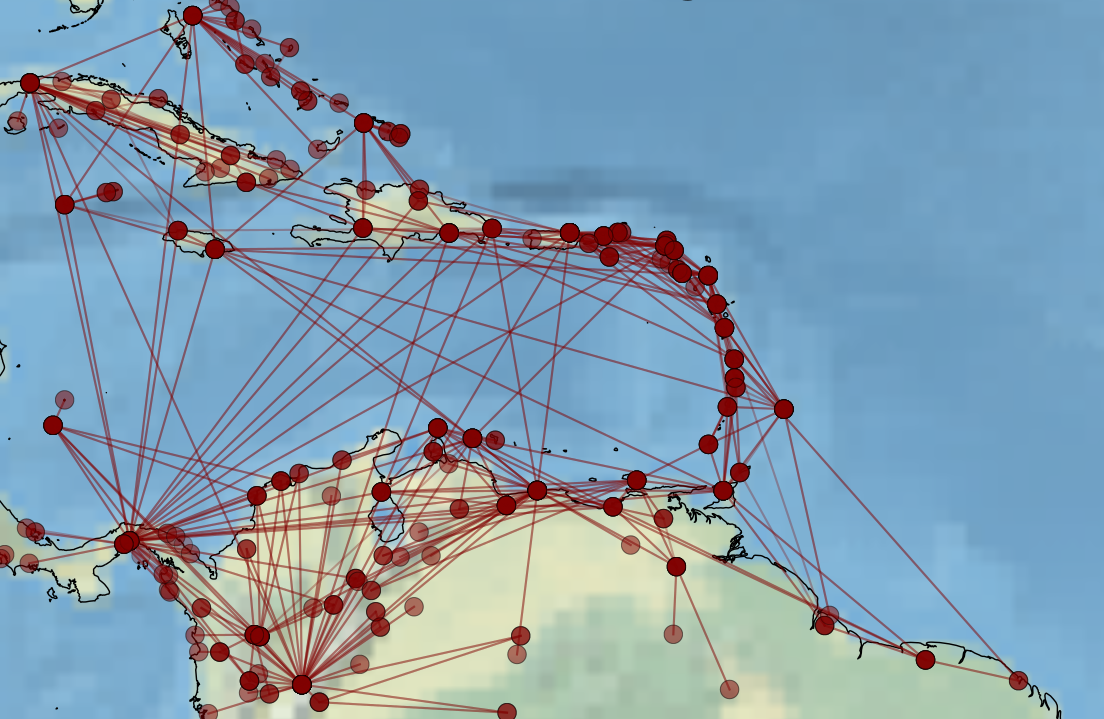
\includegraphics[width=2.7 in]{./figuras/caribbean_region}
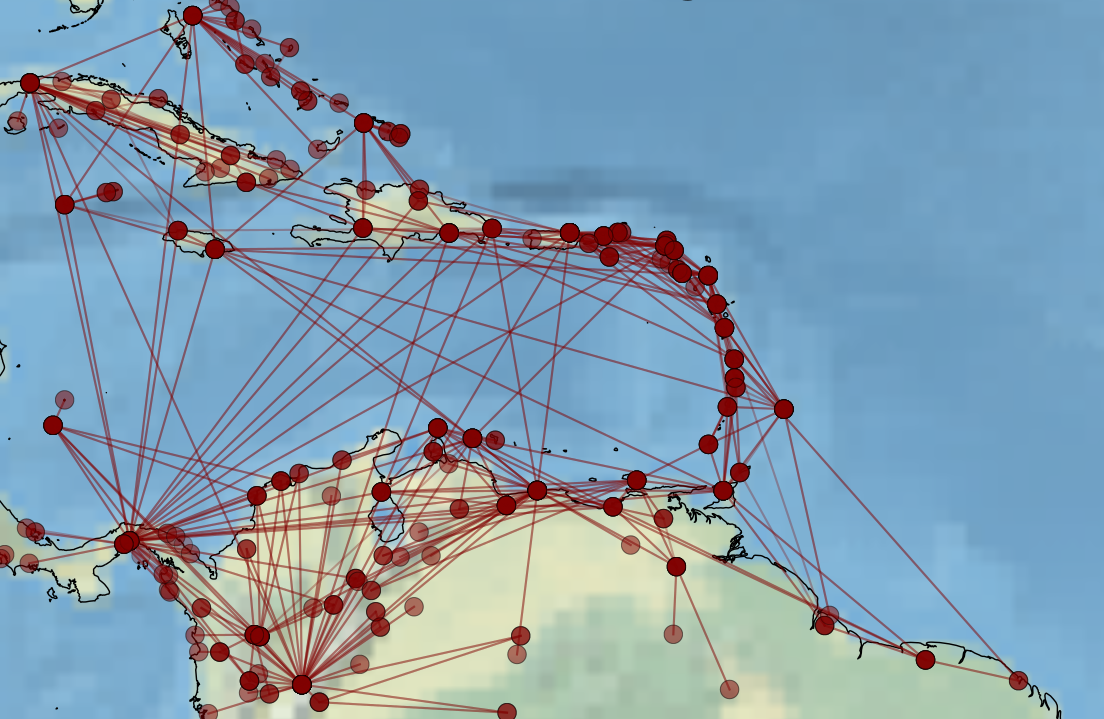
\includegraphics[width=2.3 in]{./figuras/caribbean_region} \hspace{.5cm}
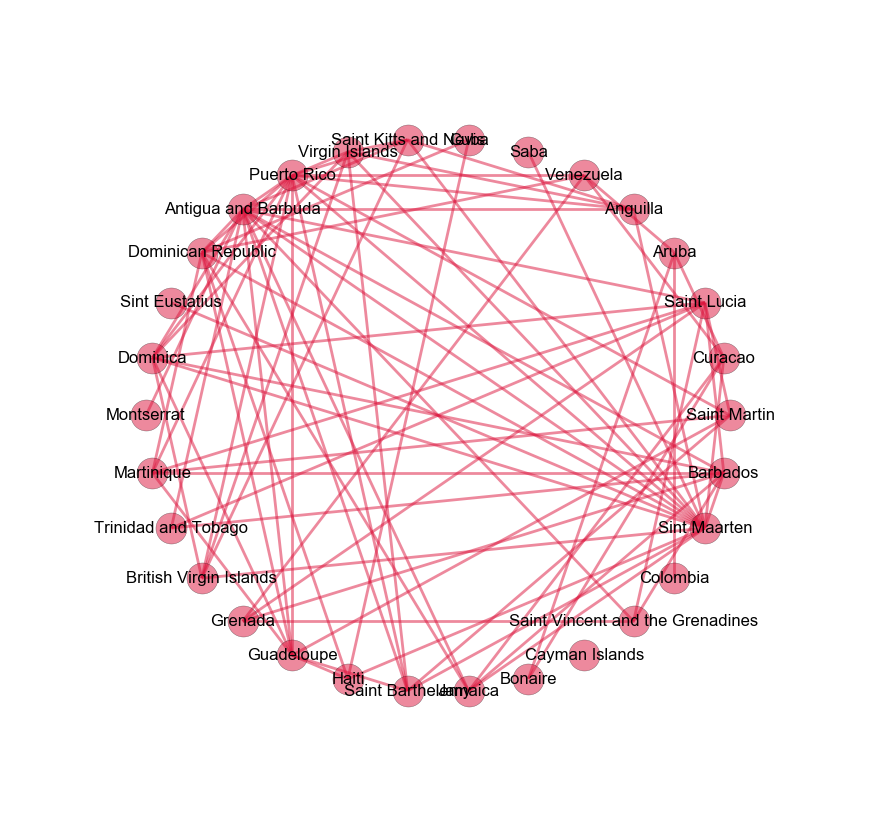
\includegraphics[width=4.7cm]{./figuras/simple_network_model_circular_and_labels_red_scen_A}
%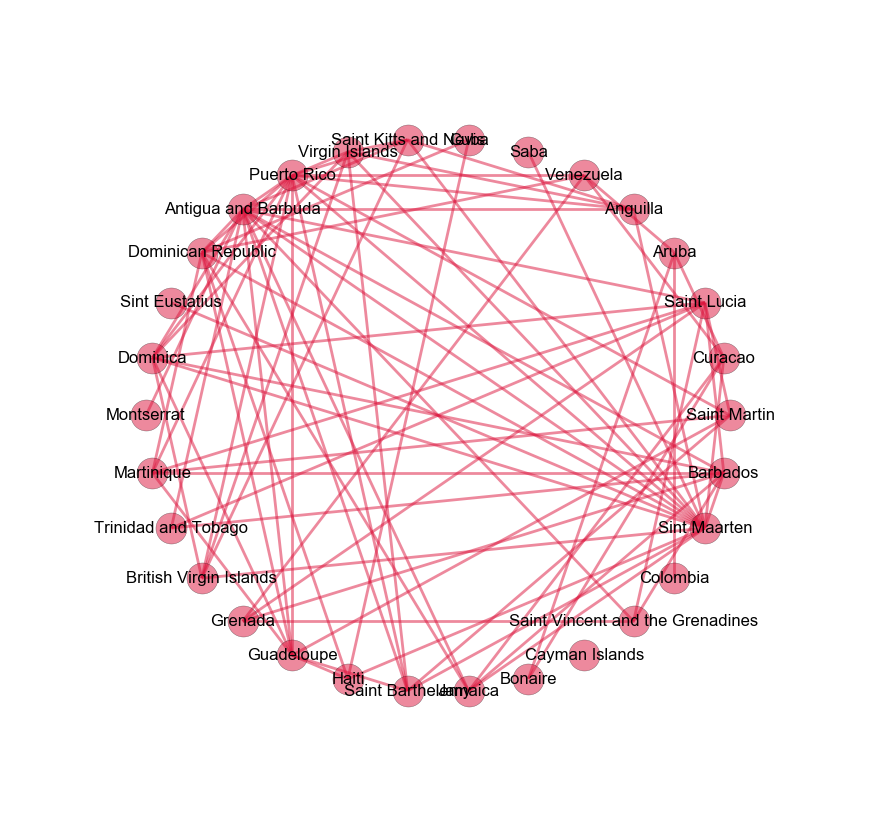
\includegraphics[width=7cm]{./figuras/simple_network_model_circular_and_labels_red_scen_A}
\caption{\small Global map showing the Caribbean area investigated (upper map). All locations and airports lying in the squared area are implemented in the SEIR network model. We show all the airport reported by openflights.org with their respective flight connections represented as links (bottom figure).}
\label{fig:world-map}
\end{figure}
%
Note that the chikungunya incidence data reported and used in this work is aggregated by political regions such as countries or territories. Since there are typically several airports within each of these political region for which we have a single aggregated data set for the infection incidence, the corresponding airports located in the same political locations have been aggregated and their respective links summed accordingly. The result is a flight network model with the number of commercial airlines that connects the regions for which we have available chikungunya data. 
\\\\
The Figure \ref{fig:network-model} shows the network model used for coupling each of the local-node SEIR submodels. Each node of the network models a location for which we have data on reported incidence of chikungunya (both confirmed and suspected cases).  The existence of a link between any two nodes indicates that there is at least one commercial airline operating between them for the time of the outbreak. 
%
Each link has associated a \textit{strength}. The link strength between any two locations is directly proportional to the number of commercial airline operating between them (i.e. the number of companies flying) and is thought as to be directly proportional to the number of passengers traveling, i.e. this is integrated as the migration rate between two nodes in the mobility network. Each node has associated a population dynamics corresponding with its own population size and is governed by the equations of the model (\ref{eq:SEIR}). 
%
The countries/islands represented as a local populations by the network nodes are the following: Puerto Rico, Dominican Republic, Jamaica, Haiti, Cuba, Cayman Islands, Bahamas, Colombia, Venezuela, Antigua and Barbuda, Barbados, Dominica, Martinique, Guadeloupe, Grenada, Virgin Islands, Saint Kitts and Nevis, Saint Lucia, Aruba, Bonaire, Curacao, Sint Eustatius, Sint Maarten, Anguilla, Trinidad and Tobago, British Virgin Islands, Saint Vincent and the Grenadines, Montserrat, Saba, and Saint Barthelemy. The list sums up 30 countries/regions.
%%
%%\begin{figure}[H]
%\begin{figure}[ht]
%\centering
%%
%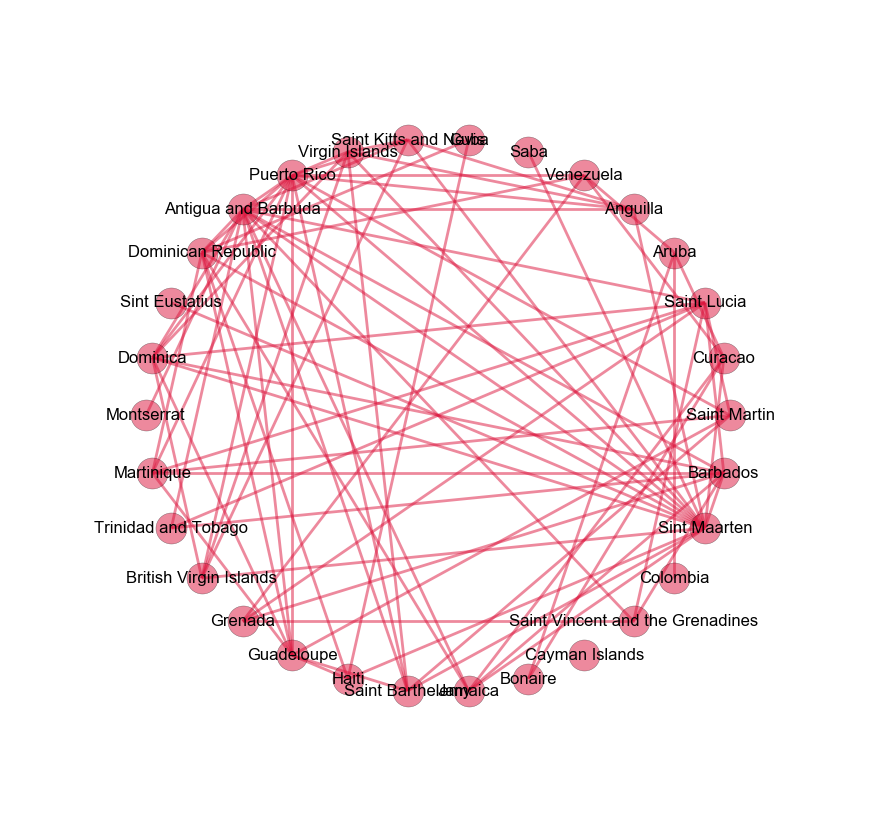
\includegraphics[width=10cm]{./figuras/simple_network_model_circular_and_labels_red_scen_A}
%%
%\caption{\small Network model of flight connection in the Caribbean. At the top the network model is rendered showing its structure where few hubs or highly connected nodes can be seen. At the bottom is the same network model organized in a circular arrangement and the names of the locations modeled by the nodes can be seen.}
%\label{fig:network-model}
%\end{figure}
%%%
%\begin{figure}[ht]
%\centering
%%\includegraphics[scale=.33]{./figures/degree_rank_plot}\\
%\vspace{.5cm}
%\includegraphics[scale=.47]{./figures/degree_distribution_plot}
%\caption{\small Degree rank and distribution plots of the flight network. In the upper panel a plot with the log-degree organized by (log) ranks is shown. Few nodes, such as Sint Marteen, Antigua and Bermuda, and Puerto Rico, have a high degree (with degrees 15, 14 and 13, respectively) while the majority has degrees between 3 to 7. An insert of the network model showing the connection topology is embed in the upper right corner. In the lower panel the network degree distribution is shown. This degree distribution looks remarkably different from a Poisson degree distribution typical of fully random networks.}
%\end{figure}
%%
\subsection*{Chikungunya incidence data}
For validating the model (\ref{eq:SEIR}) we have used the chikungunya incidence case data as reported by the Project Tycho Data for Health (\url{https://www.tycho.pitt.edu/}) for the outbreak that started in the Caribbean in December 2013. The data set reports the incidence of both confirmed and suspected cases by country/region mostly on a weekly basis. The aggregated of all these reported incidence is plotted in the Fig. \ref{fig:tycho-incidence-a}. 
%
\begin{figure}[ht]
\centering
\includegraphics[width=5.1 in, height=2 in]{./figures/observed_LT}
%\includegraphics[scale=.35]{./figures/observed_LT}
\caption{\small The incidence data. The plot shows the total aggregated number of cases (both confirmed and suspected) for the chikununya outbreak in the Caribbean for the initial 300 days period (from October 20th 2013 to August 24th 2014) according the database of the Project Tycho (https://www.tycho.pitt.edu/).}
\label{fig:tycho-incidence-a}
\end{figure}
%
\subsection*{The fitted SEIR-network model}
The parameters of the model (\ref{eq:SEIR}) for the transmission rate, the rate of moving from exposed to infectious class (the inverse of the latent period), and the recovery rate (the inverse of the infectious period), --$\beta, \sigma, \gamma$ respectively--,  have been fitted to the observed data shown in figure \ref{fig:tycho-incidence-a}. The method used is that of the least squares approach. Numerical solutions of \ref{eq:SEIR} have been produced for different values of  $\beta, \sigma$, and $\gamma$  from an initial parameter space build up out discrete intervals around initial value estimates of the parameters. The produced solutions --which are nearly continuous since they are numerical solutions of an ODE system--, have been then discretised and solutions points have been sampled to match both the number of points of the vector of observed data and their occurrences in time. 
%
In this way, the point-to-point distance between model solution vectors and the observed data vector can be computed, and both observations and model solutions be compared. 
%
A parameter space is then explored by computing solutions of the system (\ref{eq:SEIR}) with combinations of parameter values of the space and the vector distances are compared to the vector of observed data. 
%
Intervals around the initial parameter estimates are established and then discretised, that is they are divided in ten points between the interval bounds. This produce a parameter space grid of $10^3$ parameter combination points.
%
Computations of the combinations of $\beta, \sigma, \gamma$ on the parametric space grid are performed and the set of values that produces the solution with the shortest distance to the observation vector is selected and stored. This computation fulfills one iteration.
%
A new iteration is then started by setting new intervals which are 1/10th the size of the previous ones but centered around the new estimates selected and stored in the previous iteration.  Again the new (smaller) intervals are divided in ten points which serves as a new parameter space of again $10^3$ points for computing and selecting a new parameter set that again produces the shortest distance to the observation vector. 
%
This procedure is performed several times until convergence of the computed shortest distance between a solution vector and the observation vector is observed.
%
We have found that for the initial parameters estimates we use, the solution of the previously described iterative least squares fitting method converges after three iterations. That is, the fittest set of parameters $\beta,\sigma,\gamma$ is selected out of roughly $3\times10^3=3000$ points of the parameter space.
%
\\\\
Finally, we have fitted two parameter sets by the least squares method previously described to two observed time series: one time series for the very initial chikungunya observations (from 2013-10-20 to 2014-05-11), and other for the whole observed chikungunya incidence (2013-10-20 to 2014-08-24). 
%
Both time series represents the early stages of the outbreak, only that the first series accounts for the first 203 days, and the second series accounts for the first 308 days. Here we refer to them as the `short' and the `long' time series of incidence observation.
%
The initial values of the parameter set for fitting both the short and the long series is the same and is as follows: $\beta=0.81$, $\sigma=0.78$ and $\gamma=0.43$. The initial interval bounds are the initial parameter estimates plus/minus $0.5$.
%
\\\\
The Figure (\ref{fig:fitted-model-long-ts}) shows the fitted model after three iterations for the observed series of the initial 308 days of the outbreak and the Figure (\ref{fig:fitted-model-short-ts}) shows the fitted model for the initial 203 days. As previously mentioned, each of these fitting involved the computation of solutions of model (\ref{eq:SEIR}) for 1000 points (%parameter grid) three times (iterations) each.
\\\\
%% OUT
%\begin{figure}[ht]
%\centering
%\includegraphics[width=5 in]{./figures/fitted_model_iter_2_ST}
%\caption{\small Fitting of the SEIR-network model to the early observed data (from 2013-10-20 to 2014-05-11) by the least squares method. As previously described, this approach is a recursive process that selects out a defined parameter space the parameter set $\beta, \sigma, \gamma$ that produces the solution epidemic curve with the shortest distance to the observed incidence data. The recursion is done until the shortest distance converges. The observed series is depicted in red and the model solution is green. The final best fitted parameter set of the model to the observation data is then $\beta=1.21$, $\sigma=0.354$, and $\gamma=0.568$. The curves represent aggregated cases of all the observed locations for the observed time series and aggregated solutions over all individual nodes for the model simulation.}
%\label{fig:fitted-model-short-ts}
%\end{figure}
%%
\section*{Model results}
As described in the previous section, the epidemic network model (\ref{eq:SEIR}) has been parameterized and fitted by a recursive least squares method to the chikungunya aggregated case incidence data reported by the Project Tycho Data for Health \citep{TychoData} for the initial months of the outbreak in the Caribbean that started towards the end of 2013 in Saint Martin Island. 
\\\\
The Fig \ref{fig:fitted-seir} shows two fitted numerical solution (green curves) of (\ref{eq:SEIR}): one model solution fitted for the first 203 days (in the middle panel), and one model solution fitted to the first 308 days of the outbreak (bottom panel). The real aggregated observed data for that time periods is shown in the upper panel (red plot). 
%
The values of population sizes of the nodes, that represent the local populations of the model, were taken from the census information of their respective island or countries found in Wikipedia \citep{wiki:general}. 
%
\\\\
As shown in the picture (\ref{fig:fitted-seir}) the model captures the epidemic ridged curve shape exhibited by the observed time series of aggregated observations. 
%
The multi-peaked pattern of the aggregated observed incidence is made of various local single epidemic curved  peaks occurring at the several islands locations of the region that when are aggregated they render the time series shape as ridged and multi spiky (Fig \ref{fig:tycho-incidence-a}). This can be observed when plotting together the individual observed time series for locations (not shown here). A plot with a representation of the modeled individual epidemic peaks at the level  of node can be seen in the Figure(\ref{fig:wave}). 
%
The fact that all these several peaks at different nodes (and geographical locations) that are occurring at different times are all coming for a single infected individual in particular space and time point is what let us recognize the process as a spatio-temporal epidemic wave. 
%
\\\\
The model capture the same ridged pattern in the node aggregated numerical solution by being able to simulate the same pattern shown in the observed data. Specifically, the model produces a distinct spatio-temporal outbreak with single peaked simulated epidemic curves at each discrete population modeled as a node that when plotted together produce the recognizable jagged curve seen in the real data (\ref{fig:fitted-seir}). When plotted together the individual modeled epidemic curves of the nodes (not shown here) it becomes apparent that the multi-peaked shape of the aggregated model solution emerges from single peaked solutions on the several spatially apart nodes at different times. Just the same pattern  as it is displayed in the  observations. Therefore we may say that the model successfully captures the spatio-temporal mechanism observed in the data.   
\begin{figure}[ht]
\centering
%\includegraphics[width=5.3 in, height=2 in]{./figures/observed_vs_fitted_ST}
\includegraphics[scale=.5]{./figures/observed_vs_fitted_ST}\\
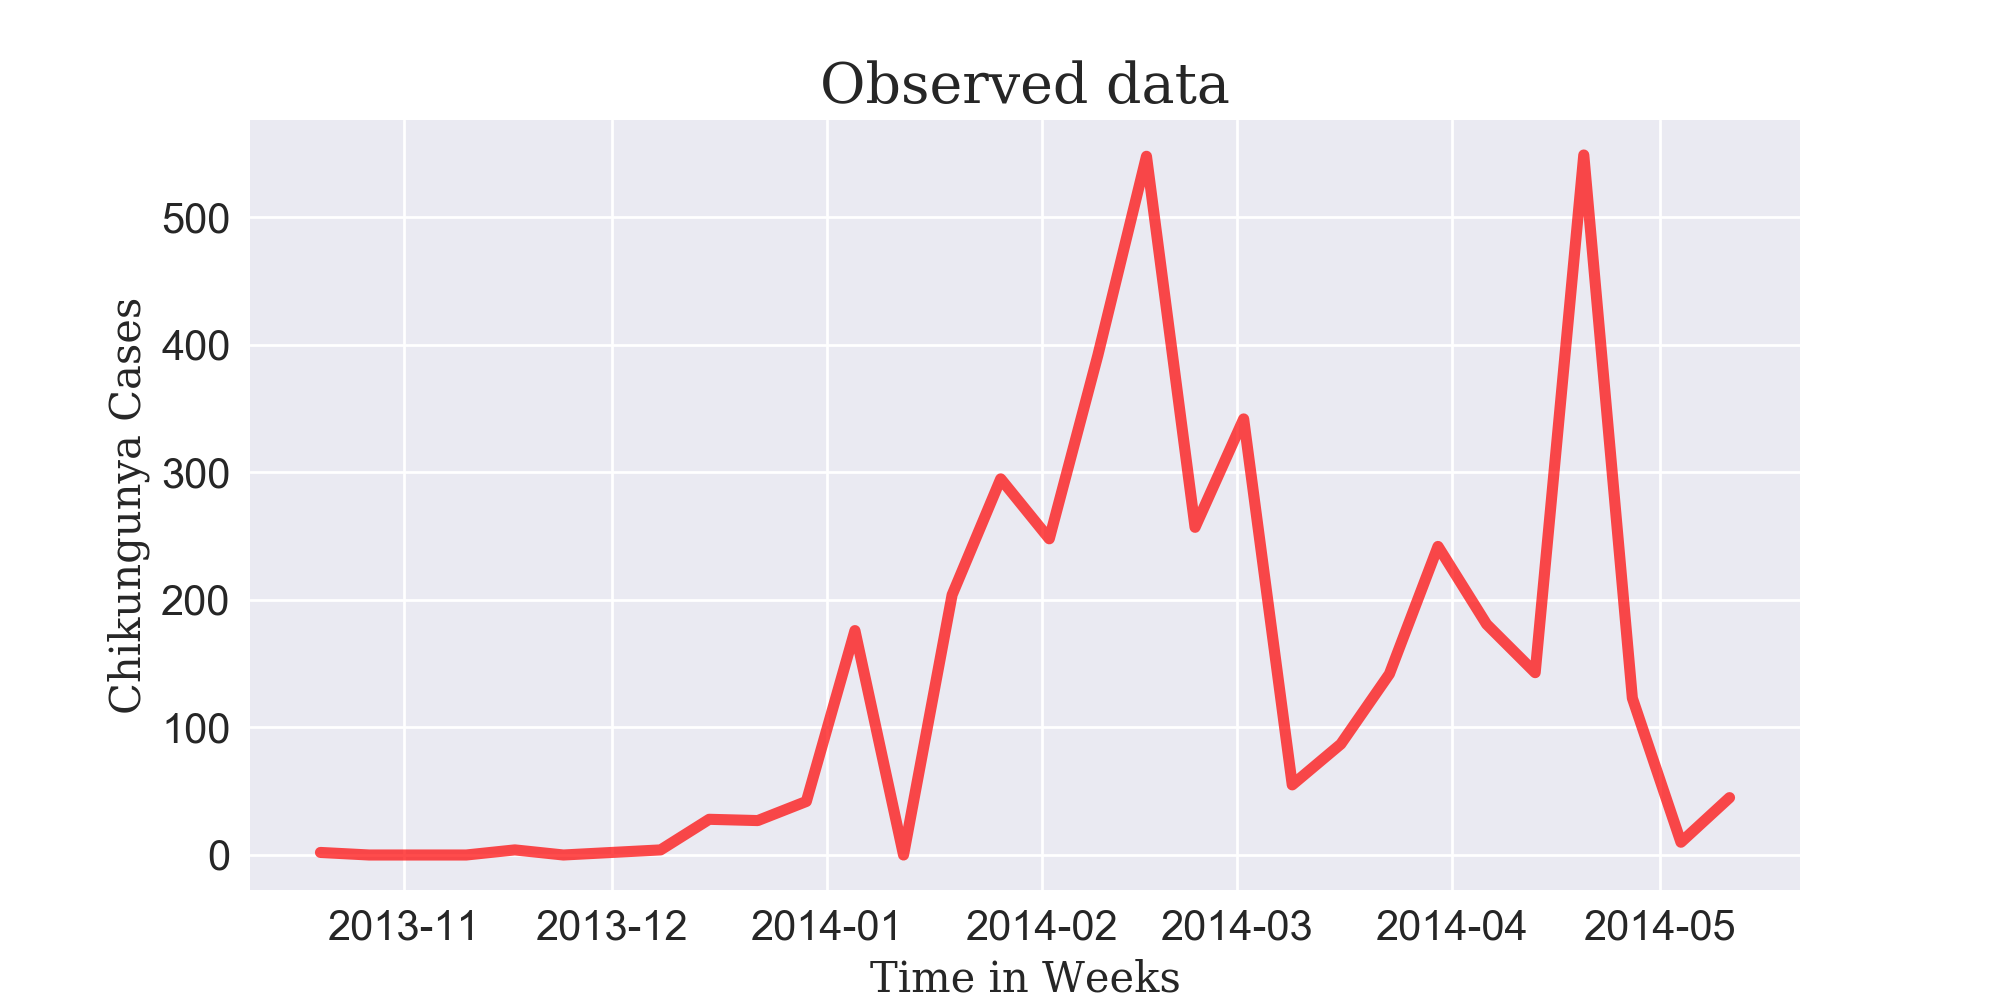
\includegraphics[scale=.5]{./figuras/observed_ST}\\
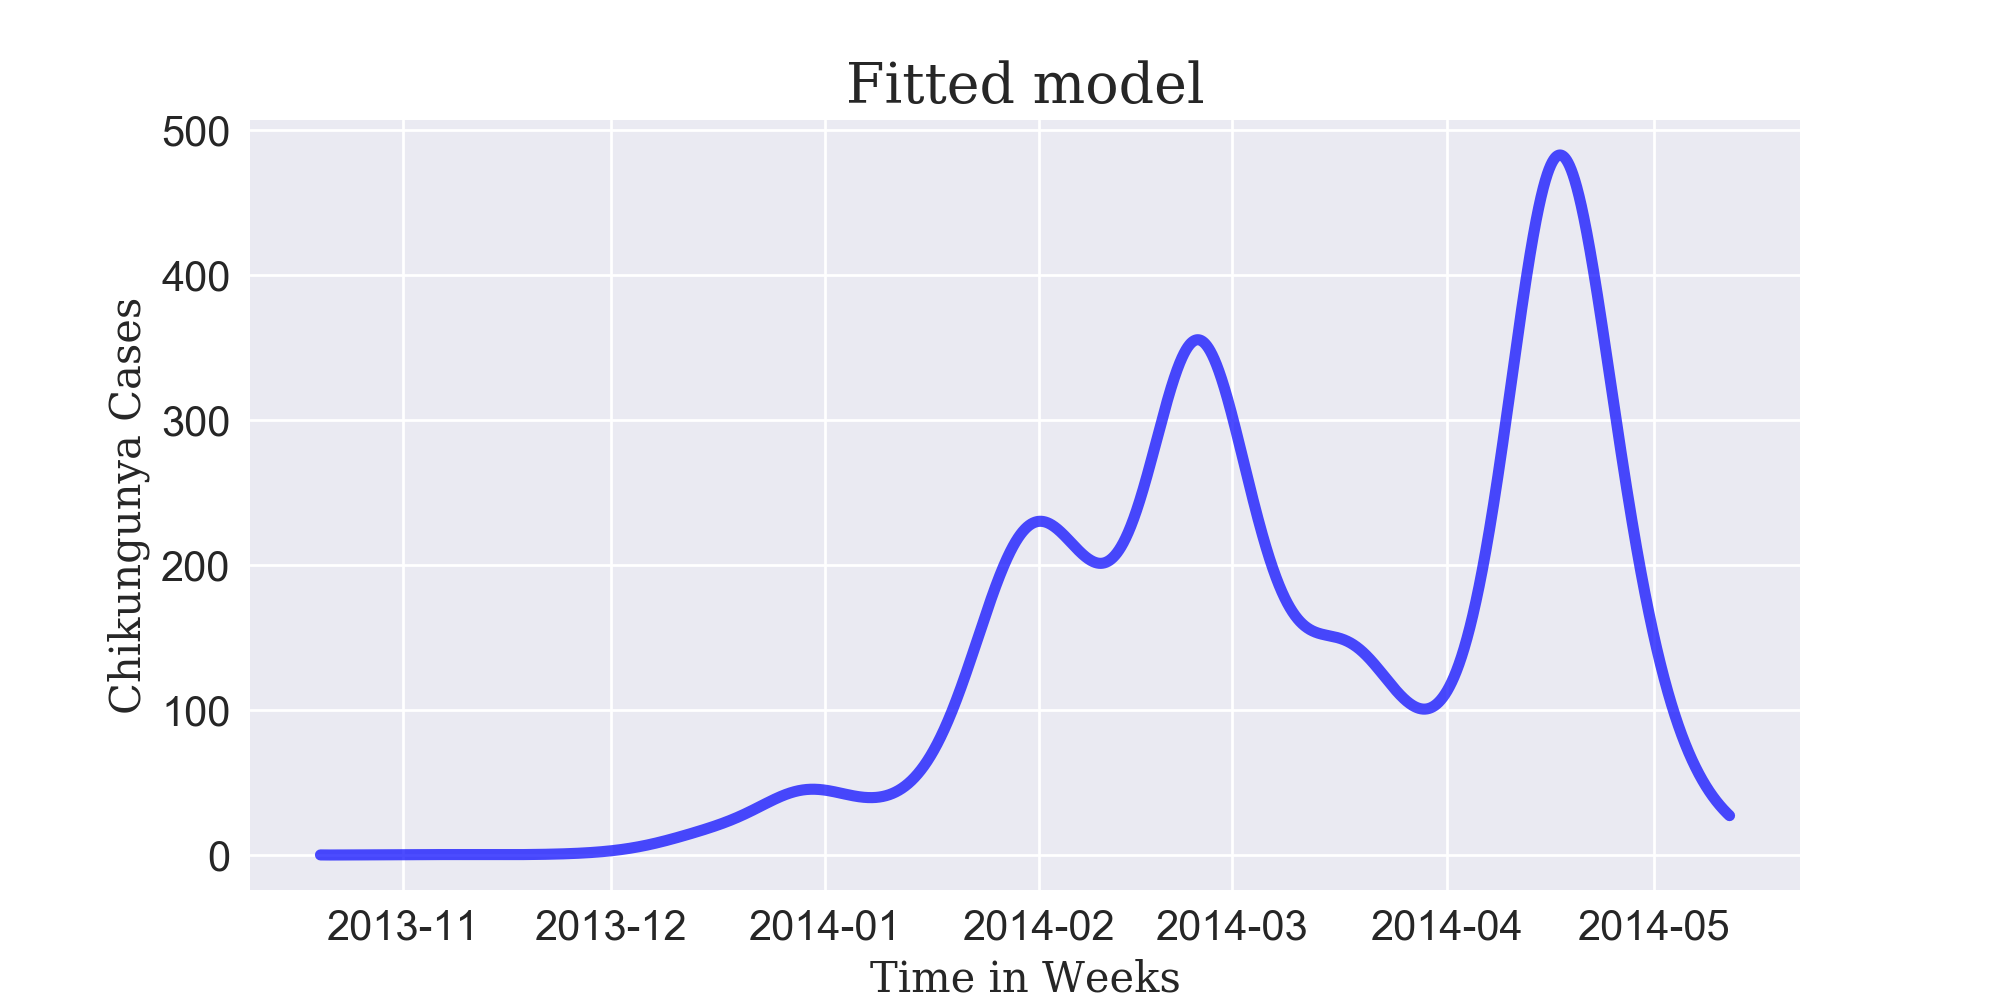
\includegraphics[scale=.5]{./figuras/fitted_ST}
\caption{\small Fitted SEIR Mobility Network model compared to observed data. The numerical solution of the model  captures the initial spreading wave of the observed aggregated incidence. The red time series shows the reported aggregated incidence data (confirmed and suspected cases) of chikungunya in the Americas during the first 308 days after first local transmission has been reported in Saint Martin Island in October 20th of 2013. The blue curve shows the SIR Network model numerical solution with the fitted parameters for the observed time series. Fitted parameters are $\beta=1.21$, $\sigma=0.354$, and $\gamma=0.568$.}
\label{fig:fitted-seir}
\end{figure}
%
\\\\
The table \ref{tab:parameters} shows the parameter values fitted for the short and long time series of observations used in the model \ref{eq:SEIR}. The epidemic wave spread has been simulated by solving numerically the SEIR network model (\ref{eq:SEIR}) with the parameters estimated as described previously. For setting the model's initial conditions population sizes for each nodes has been used corresponding with real population sizes of census information for locations these nodes represent. To simulate the observed scenario, a single infectious individual has been set at the node of Saint Martin at the epidemic day 0. These initial conditions are in accordance with the observed epidemic plot of the Chikungunya outbreak in the Americas in 2013. 
%
\begin{table}[ht]
\centering
\begin{tabular}{|c|c|c|}
\hline
\textbf{Parameter} & \textbf{Definition} & \textbf{Fitted Value} \\
\hline
$\beta$ & Transmission rate & 1.21\ding{83} / 0.448\ding{84} day$^{-1}$ \\
\hline
$\sigma$ & Incubation period & 0.354\ding{83} / 0.665\ding{84} day$^{-1}$\\
\hline
$\gamma$ & Recovery rate & 0.568\ding{83} / 0.269\ding{84} day$^{-1}$\\
\hline
\end{tabular}
\caption{\label{tab:parameters} \small Parameters of the epidemic model estimated by least squares form the observed incidence series. The values marked with (\ding{83}) corresponds to the estimates for the initial 203 days of the outbreak (see Figure \ref{fig:fitted-model-short-ts}), the values marked with (\ding{84}) corresponds to the estimates for the initial 308 days of the outbreak(see Figure \ref{fig:fitted-model-long-ts}).}
\end{table}
%
\\\\
The simulated geographical spread wave produced by the fitted model has been inspected. As mentioned, the figures (\ref{fig:fitted-model-long-ts}, \ref{fig:fitted-model-short-ts}, \ref{fig:fitted-seir}) show the model simulations of the aggregated cases for all nodes/locations. The individual simulated epidemic peaks for each nodes/locations are shown in Figure (\ref{fig:wave}). These graphics reveal the spatio-temporal structure of the epidemic wave simulated by the model by portraying the timing of the local highest epidemic peaks (for both the exposed and infectious classes). However, note that the relative magnitudes of the peaks appear similar. That is, the peaks show comparatively the same amplitude when they are not in reality; this is plotted this way for the sake of clarity. Albeit in the Figure (\ref{fig:wave}) the number of cases cannot be comparable among the different nodes/locations plots, the axis for time is identical for all of them making the timing of the local epidemic onsets and epidemic peaks comparable indeed. Thus, as earlier mentioned,  the relative time shifts of the epidemic peaks displayed by plotting the individual solutions of the nodes of the SEIR network model unveil the spatio-temporal structure of the observed epidemic wave captured by the model.
%
\begin{figure}[ht]
\centering
%\includegraphics[width=\linewidth]{map_01_global}
\includegraphics[width=5 in]{./figures/onda}
\caption{\small The epidemic wave. %\textcolor{red}{(REPHRASE THIS CAPTION?)} 
This figure shows the several simulated local epidemic curves of infected and exposed individuals (red and purple curves respectively) at each of the nodes that represent different locations in the Caribbean. At each one of the small plot-boxes the the vertical axis represents individual cases and the horizontal axis is time. Note that amplitude scales are not relative and therefore the epidemic magnitudes cannot be compared, however their timings can indeed be. The epidemic wave becomes apparent as the local epidemics peak occurs at different times. The flat curve of Cayman Islands shows no outbreak there and this is in accordance with the case that the island is not connected to the rest of the set of islands on the space domain corresponding to the selected geographical region. Therefore the Cayman Islands are not hit by the infection in our simulations. This is consistent with the observation that no chikungunya cases are reported in the Cayman Islands during the simulated time period.}  
\label{fig:wave}
\end{figure}
%
\\\\
We then use the fitted SEIR network model to assess the role of the topology of the network of connections by checking four different scenarios where we change the original topology of the network in different ways, and the initial starting node of the infection as well. We also look at a simple intervention scenario where the epidemic severity resulting of cutting off mobility at several degrees as well as cutting off at different times since detection of first infectious is measured.   
%
\\\\
We hypothesize that in an epidemic setting such as the 2013 chikungunya outbreak in the Caribbean, the geometry of the mobility pattern of the host individuals plays a definite role in the geographical spread of the disease as they are thought as the main carriers of the disease to remote locations. This hypothesis may be extended to similar settings where nearly distinct subpopulations of hosts that are loosely connected by a complex migration or mobility patterns and are naive to the infection. For this scenario we conjecture that the topology of mobility is the most important factor for the disease dynamics. This can certainly be a general case for a number of vector-borne and host-to-host infectious diseases occurring from mid to regional to global geographic scales. %, namely:
%\\\\
In the next sections we describe the scenarios.
%
\subsection*{Epidemic scenarios}
%Four scenarios has been implemented in the fitted SEIR network model in order to examine the role of the topology of the mobility network. These are described in the next paragraphs.\\\\
Four scenarios have been investigated to assess the role of the network topology in the simulated epidemic wave. The models scenarios are described as following:
\\\\
%
%%%%%%%%%%%%%%%%%%%%%%%%%%%%%%%
\textbf{a) Epidemic scenario one: Network model with randomized connections of the initial infected node}\\
In this scenario we have performed simulations of the fitted network SEIR model (\ref{eq:SEIR}) where the connections of the initial infected node (Saint Martin) has been randomized. 
%
That is, the original links that represent flight connection of Saint Martin have been randomly changed along with it corresponding strengths, the number of links of the original observed network (6) is preserved, however. 
%
Also, the rest of the connections of the network are kept the same as the original model based on the real data flights. 
%
The Fig. (\ref{fig:first-scenario}) shows 500 random simulations in which, at each single simulation, the original six connections of Saint Martin has been randomly changed. The red curve corresponds to evolution of number of aggregated infected individuals of the original network model based on the observed flight data. The curves corresponds to aggregate simulated cases of all the nodes/locations. 
%
\\\\
Visual inspection shows that disturbing the network by changing the connections of the initial node randomly, even though keeping that number of connections and preserving the rest of the network intact, can have a profound impact on the course the epidemic wave can take as shown by the many different blue epidemic curves in the Figure (\ref{fig:first-scenario}). The infection can go over many several paths producing a variety of epidemic geographic diffusion because of a seemingly small disturbance in the network structure. It is important to remark that even though each simulation is random in the sense that the links for the initial infected node are randomly rearranged for each simulation, the SEIR model itself is deterministic at the level of node/local population, so each curve is deterministic and represent a particular path trajectory of the model solution of the spread of the infection across the network nodes. Hence, since. at each single simulation, only $6$ links of the initial Saint Martin node are randomly reconnected to the rest $30 - 1 = 29$ nodes and the rest of the network is preserved unaltered, one can calculate the number of possible epidemic waves as the combinatoric number $\binom{29}{6} = 29!/29!(29-6)!$ that is, there are $475020$ possible combinations and therefore so different epidemic waves. Due to computational limitations, we have randomly chosen and simulated 500 of this possible trajectories in the hope that this is a representative sample of all possible combinations. 
\\\\ 
We can notice that the epidemic duration of the outbreak produced by original model based on the observed flight connections lies in the tail (towards the longer duration) of the distribution of epidemic durations resulting out 500 random simulations. This apparently implies that the actual observed epidemic is atypically long if compared to other possible epidemics that could be produced by relatively small random changes in the network topology of the initial infected node, in our case Saint Martin. In other words, the epidemic dynamics can be sensitive to small changes and perturbations in the topology of the network mobility.     
%
In the plots of the Figure (\ref{fig:first-scenario-stats}) statistical descriptions of the experiment of the epidemic scenario one are shown. We see that the number of infected individuals at the epidemic peak is mostly around 500 and then the number or infected and the peaks decays at what is seems an exponential manner. The histogram does not shown epidemic peaks with less than 500 infecteds however. The histograms for the time to reach epidemic peaks is not very informative though; it seems that most of the simulations peaked between 100 and 140 days after initial infection but a substantial number peaked at as earlier as 80 days and at as later as 180-200 days. 
\\\\
We have then explored a quantity that can be of interest in public epidemiology; we called the \textit{population at risk on first degree}. We define the population at risk on first degree as the size of the total population that is \textbf{directly} connected with the initial population were the infection is first reported, with this initial population included. In our context, the population risk a first degree is the sum of all populations connected (by commercial flights) to the initial infected population, including the latter. This quantity measures the total population put in peril immediately after a reported case is confirmed. The simulations for epidemic scenario one produced a histogram (Fig. \ref{fig:first-scenario-stats} left-middle panel) that reports that most of the population at risk on first degree has a size  between $\exp(10) \text{ to }\exp(11)$, i.e. $2.2\times 10^4 \text{ to } 5.99\times 10^4$ individuals. The total population of the studied geographical region is 121,913,502 individuals, therefore the model predicts a population at risk on first degree between $0.018\% \text{ to } 0.05\%$ of the population of the region. These are the average population percentages that would be at risk of immediate contagion right after the first case is reported.
\\\\
We also report three 2D histograms by contrasting pairwise the previously described ones. We report then: (a) maximum epidemic peak size vs. time to reach the peak; (b) maximum epidemic peak size vs. population at risk on first degree; and (c) time to epidemic peak vs. population at risk of first degree (Fig. \ref{fig:first-scenario-stats}). The 2D histogram (a) reports that the larger epidemic peak sizes occurred mostly between 150 to 160 days after the start of the outbreak and many peaks of 500-650 individual sizes occurred between 100 and 10 days after the start of the outbreak. 2D histogram (b) reports that the largest sizes of population at risk on first degree, between $\exp(9)$ to $\exp(11)$, occurred when the sizes of the largest epidemic peaks were at around 500-550 individuals. Finally the 2D histogram (c) reports that the highest levels of population at risk on first degrees, $\exp(10)$ to $\exp(11)$, happen when the time to reach the highest epidemic peaks is around 80 days. Population at risk of around $\exp(9)$ to $\exp(10)$ seems to be distributed more or less evenly across epidemic peaking times between 100 to 180 days. 
\\\\ 
%One can see that the randomization of the connections of the node of the initial infected node has an visible impact on the possible different paths that the infection can spread in the network, represented as the different patterns of the epidemic curves produced by the randomization. However, there seems to be still some sort of organization, since, even when we randomize the link for the initial infected node, we observe that there are some epidemic paths (i.e. the infection routes through the network) that are more frequently transited than others as the density of curves seems to be nonuniform (darker curves correspond to a greater overlap of trajectories). It is important to note that even though each simulation is random in the sense that the links or connections for the initial infected model are randomly rearranged, the SEIR model itself is deterministic, so each curve is deterministic and represent a particular path of the spread of the infection across the network nodes. It is not clear from this experiment to determine what is the precise role of the network topology in the observed pattern of the aggregated number of infected, however the observation that simulations (blue curves in Fig. \ref{fig:first-scenario}) where only the connections of a small fraction of the network have been randomly modified -namely of only the one initially infected node-, still produces length durations of outbreaks in the same range as the original unmodified network (red curve in Fig. \ref{fig:first-scenario}) suggests the the structure of the connections is important to hold the observed pattern under perturbation of the initial stages of the infection spread.
%\\\\
%
%\begin{figure}[ht]
%\centering
%%\includegraphics[width=5.1 in, height=2 in]{./figures/scenario_initial_loc_rand_conn_(250)_reps}
%\includegraphics[width=5.1 in, height=2 in]{./figures/randomized_connections_saint_martin_scenario_A}
%\caption{\small Epidemic scenario one. Randomized connections for the initial infected island. Blue curve is the SEIR model coupled with a network topology model based in flight connections data. Red curves are 500 solutions of the SEIR model coupled with the same network model but with randomized links of the initial infected node.}
%\label{fig:first-scenario}
%\end{figure}
%
%\begin{figure}[ht]
%\label{fig:first-scenario-stats}
%\centering
%\includegraphics[width=2.365 in]{./figures/infected_at_maximum_epidemic_peak_scenario_A}
%\includegraphics[width=2.365 in]{./figures/time_to_peak_scenario_A}\\
%\includegraphics[width=2.365 in]{./figures/riksy_pop_scenario_A}
%\includegraphics[width=2.365 in]{./figures/Hist1_scenario_A}\\
%\includegraphics[width=2.365 in]{./figures/Hist2_scenario_A}
%\includegraphics[width=2.365 in]{./figures/Hist3_scenario_A}
%\caption{\small Epidemic scenario one. Randomized connections for the initial infected island. Statistics over 500 simulations of the network SEIR model: a) top left is a histogram of the number of infected individuals at the epidemic peak; b) top right is a histogram of the time to reach the epidemic peak; c) middle left is a histogram of the population size at risk on first degree (the accumulated population size of all the first neighbours to the first infected node); d) middle right is a bivariate (2D) histogram of the distribution of the number of infected at the epidemic peak versus the distribution of the time to reach the peak; e) bottom left is a bivariate histogram of the distribution of the number of infecteds at the epidemic peak versus the distribution of the population at risk in the first degree; and f) bottom right is a bivariate histogram of the distribution of the time to reach the epidemic peak versus the distribution of population at risk in the first degree.}
%\end{figure}
%%
%\begin{figure}[ht]
%\centering
%%\includegraphics[width=5.1 in, height=2 in]{./figures/scenario_initial_loc_rand_conn_(250)_reps}
%\includegraphics[width=5.5 in]{./figures/histograms_B_scenario_A_sol}
%\caption{\small comments here...}
%\label{fig:first-scenario-hist}
%\end{figure}
%%
%%%%%%%%%%%%%%%%%%%%%%%%%%%%%%%%%
\textbf{b) Epidemic scenario two: Network model with initial infected node connected to all other nodes}\\
%
In this second model scenario we set the initial node, Saint Martin, to have a connection to all the other nodes in the network  while leaving the rest of the connection structure like the original topology based on the real flights. 
%
Link strengths are assigned to each of these new connections (from Saint Martin to each of the others) by randomly picking observed strengths values of the actual network. 
%
Figure \ref{fig:second-scenario} shows the epidemic curve of 500 simulations of this scenario. 
%
As one would expect, the epidemic curve of aggregated individuals exhibits a typical pattern of an outbreak of an homogeneous non-spatial model. Creating a connection of the initial infected node to all other nodes in the network produce an infection pattern close to that of an homogeneous unstructured SEIR model. This is unmistakable apparent in the plot (\ref{fig:second-scenario}) since the epidemic curve lacks the jagged structure of an explicitly spatial wave shown in the solution of the fitted models (\ref{fig:fitted-model-short-ts},\ref{fig:fitted-model-long-ts}). 
\\\\
The Figure (\ref{fig:second-scenario}) plots 500 simulations (in red) which appears as a single curve. The variation due to the randomization of the connection strengths is virtually non existent as seen in the plot. 
%
Since, in this scenario, what we (randomly) vary at each single simulation are the link strengths while keeping the the topology constant, the observation that all solution trajectories seemingly lie on a single curve  suggests that the link geometry -and not the distribution of link strengths- is the main actor in determining the spatio-temporal unfolding of the disease in the populations. That is, that topology matters more than dynamics.  
%
Therefore, this scenario serves as (i) a benchmark test to assess the role of the topology in the dynamics, and (ii) to show that the strength of the link connections seems to be irrelevant at least for the dynamics of the initial stages of an outbreak unfolding in a nearly discontinued set of naive populations. 
%
%In this second scenario, we have dramatically reduced the average path 
%length\footnote{The shortest average path length is a common measure for describing network topology and is defined as the average of the shortest paths between any two nodes in the network. Let $d(v_1,v_2)$ be the shortest distance or path between the vertices $v_1, v_2 \in V$, where $V$ is the set of all vertices or links of the network. The average (shortest) path length is defines as:
%
%$l_G = \frac{1}{n(n-1)}\sum_{i\neq j}d(v_i,v_j)$
%
%where $n$ s the number of links\citep{wiki:general}.} of the original observed network by linking the initial infected node to each of all others node of the network. The observed network based on the reported flight connection has an average (shortest) path length, $l_G^{obs} = 2.19$, whereas the average path length of the network of the is $l_G^{scen2} = 1.754 $.
\\\\
If we consider that the network topology of host mobility is important to understand the outbreak unfolding in time and space, and that the overall spread pattern is related, among other topological characteristics, with the path length \footnote{The average (shortest) path length, together with the clustering coefficient and the degree distributions of the nodes are perhaps the most relevant tenets to characterize a complex network topology. For an exhaustive introduction see \citep{mej2010networks}.} the contagion chain has to go through, then connecting the first infected node to each of every other node in the network would dramatically change the current network link geometry by reducing the shortest average path length\footnote{As said, the shortest average path length is a common measure for describing network topology and is defined as the average of the shortest paths between any two nodes in the network. Let $d(v_1,v_2)$ be the shortest distance or path between the vertices $v_1, v_2 \in V$, where $V$ is the set of all vertices or links of the network. The average (shortest) path length is defines as:

$l_G = \frac{1}{n(n-1)}\sum_{i\neq j}d(v_i,v_j)$

where $n$ s the number of links\citep{wiki:general}.}. The observed network based on the reported flight connection has an average (shortest) path length, $l_G^{obs} = 2.19$, whereas the average path length of the network of the this scenario $l_G^{scen2} = 1.754 $, which indicates that effectively the average shortest path has been decreases by connecting Saint Martin to all other nodes. This makes the contact structure of the transmission kernel to produce a disease dynamics more homogeneous from the spatial point of view. 
\\\\
Because, as discussed earlier, trajectories of the simulations of this particular scenario lie nearly on the same curve, practically no variation is then produced which render statistics futile in providing further information on the system, hence we do not take on the task to report any statistics as we do for the other cases. 
%\\\\
%The first observation \textit{(i)} -that the topology has a role in the spatial spread- can be reasoned as that by connecting the initial infected node with all other nodes, the "paths" for the disease to reach remote nodes is greatly shortened, as the average path length is definitely shortened to one 'step'.  Then we effectively observe an infection process that takes place in a homogeneous non-spatial environment, which is made clear by the appearance of a single peak epidemic curve demonstrating the classic knowledge of homogeneous SEIR processes. This occurs even while keeping the rest of the structure of the network untouched. Furthermore the patterns observed both in the real data as in the SEIR coupled with the network model based on observed flights connections (Fig. \ref{fig:fitted-seir}), namely those of the multi-peak epidemic curve and the overall epidemic length (of about 220 days) in the aggregated infecteds,  are absent and greatly reduced respectively, as a result of the shortened average path length (Fig. \ref{fig:second-scenario}).  
%On the other hand, the latter conclusion in \textit{(ii)} is a consequence of the observation that in this scenario the only randomness involved and factor that differentiates each realization of the simulation are precisely the values of the strength of the links, which are taken randomly from existent values of the observed network. And because the structure topology is fixed for each simulation's realization then the strength must be irrelevant since we observe that all trajectories overlap producing an identical epidemic pattern. In other words, the only difference between each run of a given simulation is the random assigned value of link strength, however we observe no difference in all solution trajectories, as shown in Fig. \ref{fig:second-scenario}.
%%
%\begin{figure}[ht]
%\centering
%%\includegraphics[width=5 in,draft=false]{./figures/scenario_initial_loc_full_conn_(250)_reps}
%\includegraphics[width=5 in,draft=false]{./figures/fully_connected_saint_martin_scenario_C}
%\caption{\small Epidemic scenario two. Network model with initial infected node connected to all other nodes. Blue curve is the SEIR network model based in flight connections data. Red curve are realizations of the SEIR model coupled with the same network model but with the initial infected node linked to all other nodes in the network; each of these links with strengths randomly drawn from the set of strength values of the observed network. The red curve are in fact 500 overlapped simulations that appear as a seemingly a single trajectory.}
%\label{fig:second-scenario}
%\end{figure}
%%
\\\\
%%%%%%%%%%%%%%%%%%%%%%%%%%%%%%%%%%%
\textbf{c) Epidemic scenario three: Fully randomized Erd\"{o}s-R\'{e}nyi network}\\
In the scenario 3 we investigate how a network, with the same number of nodes and approximately the same number of links as the observed flight network, but build instead by a process that produced theoretically a fully random connections between nodes, produces epidemic outbreaks. 
%
This way we can compare the disease dynamics that is produced by a theoretically complete random network with our reported network. 
%
Any deviation or difference of the spatio-temporal dynamics of the disease spread between the twos is an indication that the observed network was not designed as a full random network --not at least by a process such as the Erd\"{o}s-R\'{e}nyi algorithm  used here. 
%
Then, to build random networks keeping the constituent elements of the original observed network, i.e. both the number of nodes and links, so they would be comparable, we have used, as mentioned, the algorithm to assemble a random Erd\"{o}s-R\'{e}nyi $G(n,p)$ graph\footnote{ 
We use an algorithm to produce and uncorrelated random Erd\"{o}s-R\'{e}nyi $G(n,p)$ graph where $n$ is the number of nodes and $p$ is the probability of link formation so $n$ nodes are connected through $l$ edges which are chosen randomly from $n(n-1)/2$ possible configurations. Every pair of nodes are connected with probability $p$. The total number of edges is a random variable with expected value $np(n-1)/2$ hence $p = 2l/(n(n-1))$. Thus introducing the observed number of nodes and observed number of links as $n,l$ for the expression for $p$ we obtain our probability of connection to generate a comparable fully random network to that of the observed network.}, see \citep{mej2010networks, jackson2010social} for details.
\\\\
For each simulation we generate a $G(n,p)$ random graph by using the number of nodes $n$ of the observed network and the corresponding link formation probability $p$ that corresponds to the observed number of links and number of nodes. We then assign to the new network the nodes properties of local population sizes that correspond to the locations of the real network. We seed an infected individual at the Saint Martin node and simulate an epidemic. We save the generated artificial outbreak and proceed to repeat to generate a new random simulation.
% 
The Figure (\ref{fig:third-scenario}) shows the of the curves of infected individuals of 500 simulations (in red) of a fully randomized network based in the network model of observed flight connections. The number of links are kept the same as the observed network based on the flights data, but they are rearranged in a random manner according the Erd\"{o}s-R\'{e}nyi algorithm. 
%
%That is, for the set of existing links of the observed network, each one is, in the new instance network, reassigning to a pair of nodes by drawing randomly two existing nodes of the observed network. The result is a simulation composed by realizations consisting of newly formed random networks with the same number of nodes (along with its population sizes) and the same number of links (along with their strength values). A simulation of 250 realizations is shown in Fig. \ref{fig:third-scenario}. 
%
\\\\
%\begin{figure}[ht]
%\centering
%%\includegraphics[width=5 in]{./figures/scenario_fully_random_network(250)_reps}
%\includegraphics[width=5 in]{./figures/Erdos-Renyi_scenario_D}
%\caption{\small Epidemic scenario three. Fully randomized Erd\"{o}s-R\'{e}nyi network. Red curve is the SEIR model coupled with a network topology model based in flight connections data. Blue curves are 500 realizations of the SEIR model coupled with 200 different random networks build with the same number of links and nodes as the network based on the flight observed data along with their respective population sizes for the nodes, and link strengths for the links.}
%\label{fig:third-scenario}
%\end{figure}
%%
%\begin{figure}[ht]
%\centering
%%\includegraphics[width=\linewidth]{map_01_global}
%\includegraphics[width=2.365 in,draft=false]{./figures/infected_at_maximum_epidemic_peak_scenario_D}
%\includegraphics[width=2.365 in,draft=false]{./figures/time_to_peak_scenario_D}\\
%\includegraphics[width=2.365 in,draft=false]{./figures/riksy_pop_scenario_D}
%\includegraphics[width=2.365 in,draft=false]{./figures/Hist1_scenario_D}\\
%\includegraphics[width=2.365 in,draft=false]{./figures/Hist2_scenario_D}
%\includegraphics[width=2.365 in,draft=false]{./figures/Hist3_scenario_D}
%\label{fig:third-scenario-stats}
%\caption{\small Epidemic scenario three. Fully randomized Erd\"{o}s-R\'{e}nyi network. Statistics over 500 realizations of the SEIR model coupled with the network model: a) top left is a histogram of the number of infected individuals at the epidemic peak; b) top right is a histogram of the time to reach the epidemic peak; c) middle left is a histogram of the population size at risk on first degree (the accumulated population size of all the first neighbours to the first infected node); d) middle right is a bivariate (2D) histogram of the distribution of the number of infected at the epidemic peak versus the distribution of the time to reach the peak; e) bottom left is a bivariate histogram of the distribution of the number of infecteds at the epidemic peak versus the distribution of the population at risk in the first degree; and f) bottom right is a bivariate histogram of the distribution of the time to reach the epidemic peak versus the distribution of population at risk in the first degree.}
%\end{figure}
%%%
%\begin{figure}[ht]
%\centering
%%\includegraphics[width=5.1 in, height=2 in]{./figures/scenario_initial_loc_rand_conn_(250)_reps}
%\includegraphics[width=5.5 in]{./figures/histograms_B_scenario_D_sol}
%\caption{\small Scenario 3 (commnets...)}
%\label{fig:third-scenario-hist}
%\end{figure}
%%
%
In comparison to the outbreak in observed network, the outbreaks simulated on the randomized network exhibit a reduced overall epidemic length. Only 5 simulations out of 500 had longer durations than the observed network. 
%
If we conjecture that the observed flight connection network was not generated as a fully random network, because the establishment of airline connections, by common sense, does not follow random rules but rather the decisions to make connections are far from arbitrary, then we would expect qualitatively differences between epidemics produced by completely random networks and the observed network based on the flights pattern. 
% 
Accordingly, we expected fully random networks with exponential degree distributions to have an average shortest path lengths shorter than these path lengths found in natural networks with a more organized topology that bear a mix between structured and random link geometries, and skewed degree distributions \citep{mej2010networks,jackson2010social}. 
%
This would explain the significant shorter epidemic durations of the full random model as compared with the observed model as evident in the Figure (\ref{fig:third-scenario}). Shortest average paths of the fully random networks would be more efficient to diffuse the disease in the network yielding faster outbreaks with shorter extinction times and larger epidemic peaks, which is what we observe in the plots of (\ref{fig:third-scenario}). 
%
Additionally, the histograms of Figure (\ref{fig:third-scenario-stats}) reveal that the epidemic sizes are in general larger than any of the epidemic scenarios investigate here. The most common epidemic peak sizes observed in the Erd\"{o}s-R\'{e}nyi model are about 800-1000 individuals (typical peaks of scenario 1 is around 500 individuals), and the more frequent times to peak oscillates from 80 to 120 days (which are significant shorted that the values of 100 to 140 days for scenario 1). The typical population sizes at risk on first degree lies between $\exp(10)$ to $\exp(12)$ (which is significant larger than the values $\exp(10)$ to $\exp(11)$ for scenario 1). According the 2D histograms we can see that the largest epidemic peaks (900 to 1100 individuals) occurs when the time to reach these peaks are about 90 to 110 days from the start of the epidemic. The highest values for population size at risk on first degree (around $\exp(11)$ and more) occurs when the maximum epidemic peak is around 800-900 individuals. And finally, these highest values of population at risk on fist degree coincide when the times to epidemic peaks are at 60 days from the start of the infection.
\\\\
%%%%% 
\textbf{d) Epidemic scenario four: Initial infected node location chosen randomly.}\\
In this scenario the topology of the network model based on the flight connections is unmodified but the initial infected location or node is chosen randomly for each simulation realization. The result of a simulation of 250 random realizations is show in Fig. \ref{fig:fourth-scenario}. We can notice that both epidemic patterns observed in the outbreak produced by starting in the node corresponding with the real observation Saint Martin, i.e. multi-peak curves of aggregated infecteds and overall epidemic length, are still reproduced in this scenario. 
\\\\
Since the topology of the network is not modified and only the starting point of the infection process is (randomly) changed, the observation that the epidemic patterns are retained in the simulations indicate that the actual topology has an important role in the spatio-temporal deployment of the CHIKV in the first stages of the outbreak in the Caribbean.  We then can consider this model to investigate some intervention scenarios to learn about the conditions that might help to mitigate similar outbreaks in future situations.
%
%%\\\\
%\begin{figure}[ht]
%\centering
%%\includegraphics[width=5 in,draft=false]{./figures/scenario_initial_loc_rand_(250)_reps}
%\includegraphics[width=5 in,draft=false]{./figures/randomized_initial_seed_scenario_B}
%\caption{\small Epidemic scenario four. Initial infected node location chosen randomly. Blue curve is the SEIR model coupled with a network topology model based in flight connections data. Red curves are 500 simulation of the SEIR model coupled with the same network model but with randomly chosen initial infected node.}
%\label{fig:fourth-scenario}
%\end{figure}
%%
%%
%\begin{figure}[ht]
%\centering
%%\includegraphics[width=\linewidth]{map_01_global}
%\includegraphics[width=2.365 in,draft=false]{./figures/infected_at_maximum_epidemic_peak_scenario_B1}
%\includegraphics[width=2.365 in,draft=false]{./figures/time_to_peak_scenario_B1}\\
%\includegraphics[width=2.365 in,draft=false]{./figures/riksy_pop_scenario_B1}
%\includegraphics[width=2.365 in,draft=false]{./figures/Hist1_scenario_B1}\\
%\includegraphics[width=2.365 in,draft=false]{./figures/Hist2_scenario_B1}
%\includegraphics[width=2.365 in,draft=false]{./figures/Hist3_scenario_B1}
%\label{fig:fourth-scenario-stats}
%\caption{\small Epidemic scenario four. Initial infected node location chosen randomly. Statistics over 500 simulations of the SEIR model coupled with the network model: a) top left is a histogram of the number of infected individuals at the epidemic peak; b) top, right is a hostogram of the time to reach the epidemic peak; c) middle left is a histogram of the population size at risk on first degree (the accumulated population size of all the first neighbours to the first infected node); d) middle right is a bivariate (2D) histogram of the distribution of the number of infected at the epidemic peak versus the distribution of the time to reach the peak; e) bottom left is a bivariate histogram of the distribution of the number of infecteds at the epidemic peak versus the distribution of the population at risk in the first degree; and f) bottom right is a bivariate histogram of the distribution of the time to reach the epidemic peak versus the distribution of population at risk in the first degree.}
%\end{figure}
%%
%%
%\begin{figure}[ht]
%\centering
%%\includegraphics[width=5.1 in, height=2 in]{./figures/scenario_initial_loc_rand_conn_(250)_reps}
%\includegraphics[width=5.5 in]{./figures/histograms_B_scenario_B_sol}
%\caption{\small Scenario 4 (commnets...)}
%\label{fig:fourth-scenario-hist}
%\end{figure}
%%


\begin{center}
    \begin{tabular}{| c | p{3cm} | p{3cm}| p{3cm} |}
    \hline
    Scenario & Infecteds at Peak (mean/sd)& Time to Peak (days mean/sd) & Accumulated Infecteds at peak (mean/sd) \\ \hline
    Scenario 1 & 577.2/104.1  & 129.6/30.2 & 363192.2/133459.7 \\ \hline
    Scenario 2 & 1032.4/0.0 * & 80.0/0.0 *  & 338688.1/0.0 * \\ \hline
    Scenario 3 & 734.8/166.6 & 103.1/18.6 & 327661.9/97152.9 \\ \hline
    Scenario 4 & 497.2/104.9 & 152.8/44.0 & 439021.1/129005.4 \\ 
    
    \hline
    \end{tabular}
\end{center}

%
\subsection*{Intervention scenarios}
The calibrated and parameterised model can be use to explore simple cases of interventions in order to mimic the consequences of the decisions taken and public policies and strategies triggered in face of an icoming epidemic event.   
The plots shown here represent the effect of intervention actions on the SEIR network model of chikungunya for the Caribbean that started in November 2013 based in a set of coupled ODEs by means of a network topology that resembles the real traffic of commercial airline flights. 
\\\\
The intervention are based on evident actions that decision makers controlling air traffic can take, that is reducing flights numbers or flights activity at some point in time after the outbreak has been recognized. This is modelled here as a reduction in the percentage or level of the connection strength of the air traffic network model at different times after day one of the outbreak, i.e. when a first infected is accounted. 
\\\\
Eleven levels --from 0\%, 10\%, 20\%, $\cdots$, \%100-- of ``intervention actions'' have been simulated. For example 0\% means no intervention and the interaction strength is the same as the fitted model, 10\% means that there is a 10\% of reduction of the link strengths in the network, and so on.
\\\\
Sixteen times to implement an intervention action after outbreak day one has been simulated to investigate the effect of the response quickness of the intervention on the overall outbreak. The plots represent the time evolution of the aggregated infected in all the nodes/islands/populations of the Caribbean network.


\begin{figure}
\centering
\subfloat[Interventions at day 5]{
  \includegraphics[width=65mm]{./figures/aggregated_infecteds_PRE_plus_POST_INTERVENTION_day_(5).png}
}
\subfloat[Interventions at day 10]{
  \includegraphics[width=65mm]{./figures/aggregated_infecteds_PRE_plus_POST_INTERVENTION_day_(10).png}
}
\hspace{0mm}
\subfloat[Interventions at day 20]{
  \includegraphics[width=65mm]{./figures/aggregated_infecteds_PRE_plus_POST_INTERVENTION_day_(20).png}
}
\subfloat[Interventions at day 40]{
  \includegraphics[width=65mm]{./figures/aggregated_infecteds_PRE_plus_POST_INTERVENTION_day_(40).png}
}
\hspace{0mm}
\subfloat[Interventions at day 60]{ 
  \includegraphics[width=65mm]{./figures/aggregated_infecteds_PRE_plus_POST_INTERVENTION_day_(60).png}
}
\subfloat[Interventions at day 80]{
  \includegraphics[width=65mm]{./figures/aggregated_infecteds_PRE_plus_POST_INTERVENTION_day_(80).png}
  }
\hspace{0mm}
\subfloat[Interventions at day 100]{
  \includegraphics[width=65mm]{./figures/aggregated_infecteds_PRE_plus_POST_INTERVENTION_day_(100).png}
}
\subfloat[Interventions at day 120]{
  \includegraphics[width=65mm]{./figures/aggregated_infecteds_PRE_plus_POST_INTERVENTION_day_(120).png}
}
\hspace{0mm}
\subfloat[Interventions at day 140]{   %
  \includegraphics[width=65mm]{./figures/aggregated_infecteds_PRE_plus_POST_INTERVENTION_day_(140).png}
}
\subfloat[Interventions at day 150]{
  \includegraphics[width=65mm]{./figures/aggregated_infecteds_PRE_plus_POST_INTERVENTION_day_(150).png}
}
\caption{\small The effect of several levels of interventions at different times of the epidemic. The outcome of the SEIR network model fitted for the short data time series (\ref{fig:fitted-model-short-ts}) is inspected under a simple intervention action such as mobility restriction by halting the flight traffic. 
%
We have simulated this intervention by decreasing the original migration rates at 10 different degrees of their original values; i.e. from 100\% of the original migration rates which is the full original migration rate, going trough 90\%, 80\%, ... all the way down to 0\% that corresponds to no migration and isolation of the nodes. Remind that migration rates are modeled as the link strengths in the network model. Therefore in the scenario of 0\% of the migration rates, we have a completely disconnected network depicting thus the maximum degree of intervention. The red curves plot the modeled chikungnya case incidence prior-intervention. The small black arrow points the exact time where the intervention has been done. The action of intervening by cutting down the migration rates is then hold. The consequences of the different degrees on interventions are depicted by the color gradation of the epidemics curves: the curves colored  towards the green have undergone less intervention (that is migration rate less decreased) with the greener curve having no intervention at all. on the other hand, the curves with colors turning towards the blue have undergone more intervention, and the bluest of them having complete intervention and rendering the network into a set of completely isolated nodes.}
\end{figure}

\section*{Discussion}
The Discussion should be succinct and must not contain subheadings.
%

\bibliography{sample}{}
\bibliographystyle{plain}
\end{document}


